In this section, we discuss the performance and scalability of a
gravitational $N$-body simulation code implemented using FDPS. Some
results in this scetion have been published in \citet{2015FDPS}. The
code is essentially the same as the sample code described in
section~\ref{sec:samplecode}, except for the following two differences
in the user code for the calculation of the interaction. First, to
improve the accuracy, we used the expansion up to the quadrupole
moment, instead of the monopole-only one used in the sample
code. Second, we used the highly optimized kernel developed using SIMD
builtin functions, instead of the simple one in the sample code.

We apply this code for the simulation of the Milky Way-like galaxy,
which consists of a bulge, a disk, and a dark matter halo. For
examples of recent large-scale simulations,
see \citet{2011ApJ...730..109F}
and \citet{Bedorf:2014:PGT:2683593.2683600}.

The initial condition is the Milky Way model, which is the same as
that in \citet{Bedorf:2014:PGT:2683593.2683600}. The mass of the bulge
is $4.6 \times 10^9 M_\odot$, and it has a spherically-symmetric
density profile of the Hernquist model \citep{1990ApJ...356..359H}
with the half-mass radius of $0.5$~kpc. The disk is an axisymmetric
exponential disk with the scale radius of $3$~kpc, the scale height of
$200$~pc and the mass $5.0 \times 10^{10}M_\odot$. The dark halo has
an Navarro-Frenk-White (NFW) density
profile \citep{1996ApJ...462..563N} with the half-mass radius of
$40$~kpc and the mass of $6.0 \times 10^{11} M_\odot$. In order to
realize the Milky Way model, we used
GalacticICS \citep{2005ApJ...631..838W}. For all simulations in this
section, we adopt $\theta=0.4$ for the opening angle for the tree
algorithm. We set the average number of particles sampled for the
domain decomposition to 500.

%We adopt $\theta=0.4$ for the opening angle for the tree algorithm.
%In this paper, we present the weak-scaling performance of the code
%with FDPS. Therefore we fixed the number of particles per node to
%$2.1$ million and measured the performance for number of nodes in the
%range of 128 to 16384.  For the Plummer model, performance measurement
%for up to $76544$ has been finished at the time of writing. The
%obtained performance numbers are quite similar for these two models.

Figure~\ref{fig:evolutiondisk} illustrates the time evolution of the
bulge and disk in the run with $512$ nodes on the K computer. The disk
is initially axisymmetric. We can see that spiral structure develops
(0.5 and 1 Gyrs) and a central bar follows the spiral (1 Gyrs and
later). As the bar grows, the two-arm structure becomes more visible
(3 Gyrs).

\begin{figure}
  \begin{center}
    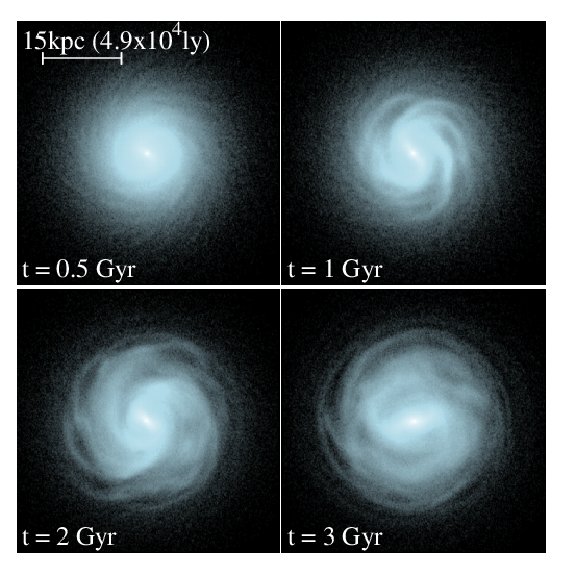
\includegraphics[width=8cm]{figure/disk.eps}
  \end{center}
  \caption{
  Face-on surface density maps of the bulge and disk.
  }
  \label{fig:evolutiondisk}
\end{figure}

Figure~\ref{fig:disk_weak} shows the measured weak-scaling
performance. We fixed the number of particles per core to 266,367 and
measured the performance for the number of cores in the range of 4096
to 663,552 on the K computer, and in the range of 32 to 2048 on
XC30. We can see that the measured efficiency and scalability are both
very good. The efficiency is more than 50\% for the entire range of
cores on the K computer. The efficiency of XC30 is a bit worse than
that of the K computer. This difference comes from the difference of
two processors. The Fujitsu processor showed higher efficiency, while
the Intel processor has 5.2 times higher peak performance per core. We
can see that the time for domain decomposition increase as we increase
the number of cores. The slope is around 2/3 as can be expected from
our current algorithm discussed in section \ref{sec:decomposition}.

%, because of the difference of SIMD vector
%length. Since the SIMD vector length on XC30 is four times longer than
%that on the K computer, the efficient usage of SIMD units on XC30 is
%more difficult than that on the K computer. We can see the increase of
%time spent for domain decomposition is slower than that of the number
%of cores. This is because that we use parallelized domain
%decomposition described in section \ref{sec:decomposition}.

Figure~\ref{fig:disk_strong} shows the measured strong-scaling
performance. We fixed the total number of particles to $550$ million
and measured the performance for 512 to 32768 cores on K computer and
256 to 2048 cores on XC30. We can also see the measured efficiency and
scalability are both very good, for the strong-scaling performance.



%The efficiency is about 50\% for the entire range of nodes.

%Figure~\ref{fig:disk_strong} shows the breakups of the measured
%strong-scaling performance. 

%Wallclock time shows slight increase for larger number of
%nodes, but this is due to the increase of the calculation cost and not
%due to the degradation of the efficiency.

%Figure~\ref{fig:disk_strong} shows the measured strong-scaling
%performance. We fixed the number of particles per node to $2.1$ million particles. We
%can see the measured efficiency and scalability are both very
%good. Efficiency is very close to 50\%, for both models and for the
%entire range of nodes. Wallclock time shows slight increase for larger
%number of nodes, but this is due to the increase of the calculation
%cost and not due to the degradation of the efficiency.

\citet{Bedorf:2014:PGT:2683593.2683600}
reported the wallclock time of 4 seconds for their 27-billion particle
simulation on the Titan system with 2048 NVIDIA Tesla K20X, with the
theoretical peak performance of 8PF (single precision, since the
single precision was used for the interaction calculation). This
corresponds to 0.8 billion particles per second per petaflops. Our
code on K computer requires 15 seconds on 16384 nodes (2PF theoretical
peak), resulting in 1 billion particles per second per
petaflops. Therefore, we can conclude that our FDPS code achieved the
performance slightly better than one of the best codes specialized to
gravitational $N$-body problem.

\begin{figure}
  \begin{center}
    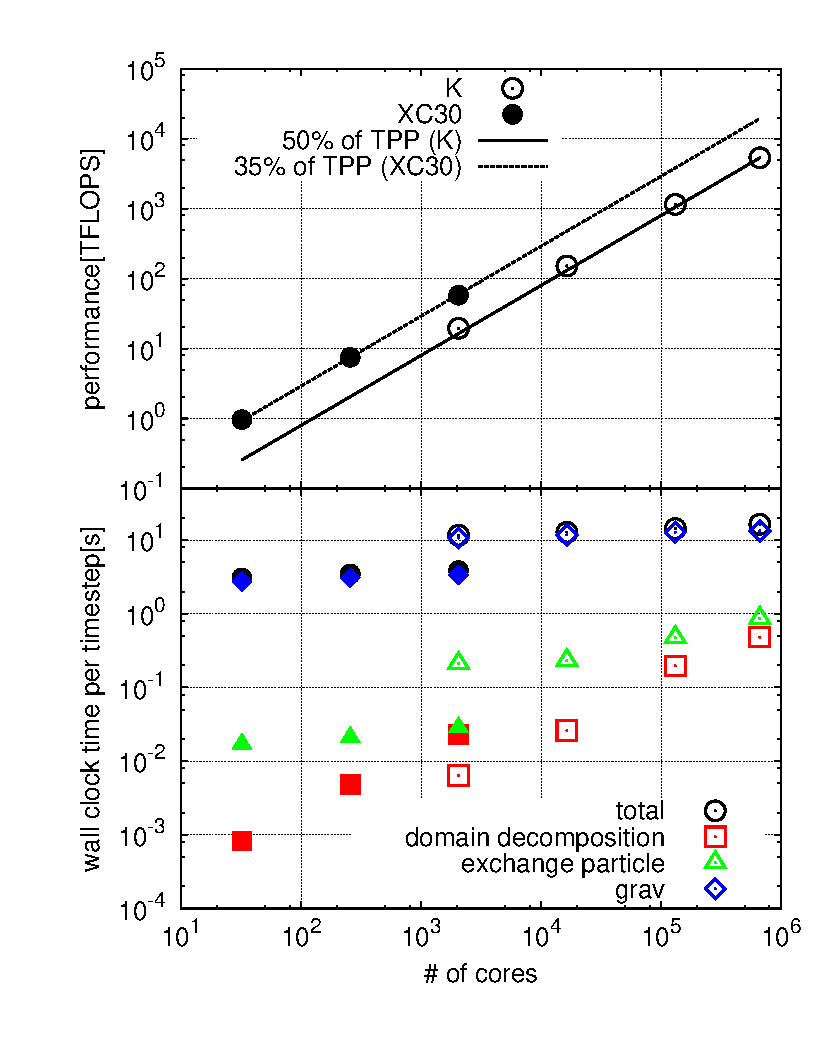
\includegraphics[width=8cm]{figure/disk_weak.eps}
  \end{center}
  \caption{
  
    Weak-scaling performance of the gravitational $N$ body code. The
    speed of the floating-point operation (top) and wallclock time per
    one timestep (bottom) are plotted as functions of the number of
    cores. Open and filled symbols indicate the performances of K
    computer and cray XC30, respectively. In the top panel, the solid
    line indicates 50\% of the theoretical peak performance of K
    computer and the dotted line indicates 35\% of the theoretical
    peak performance of XC30. In the bottom panel, time spent for the
    interaction calculation (diamond), the domain decomposition
    (square) the exchange particles (triangle) are also shown.
    
    } \label{fig:disk_weak}
\end{figure}

\begin{figure}
  \begin{center}
    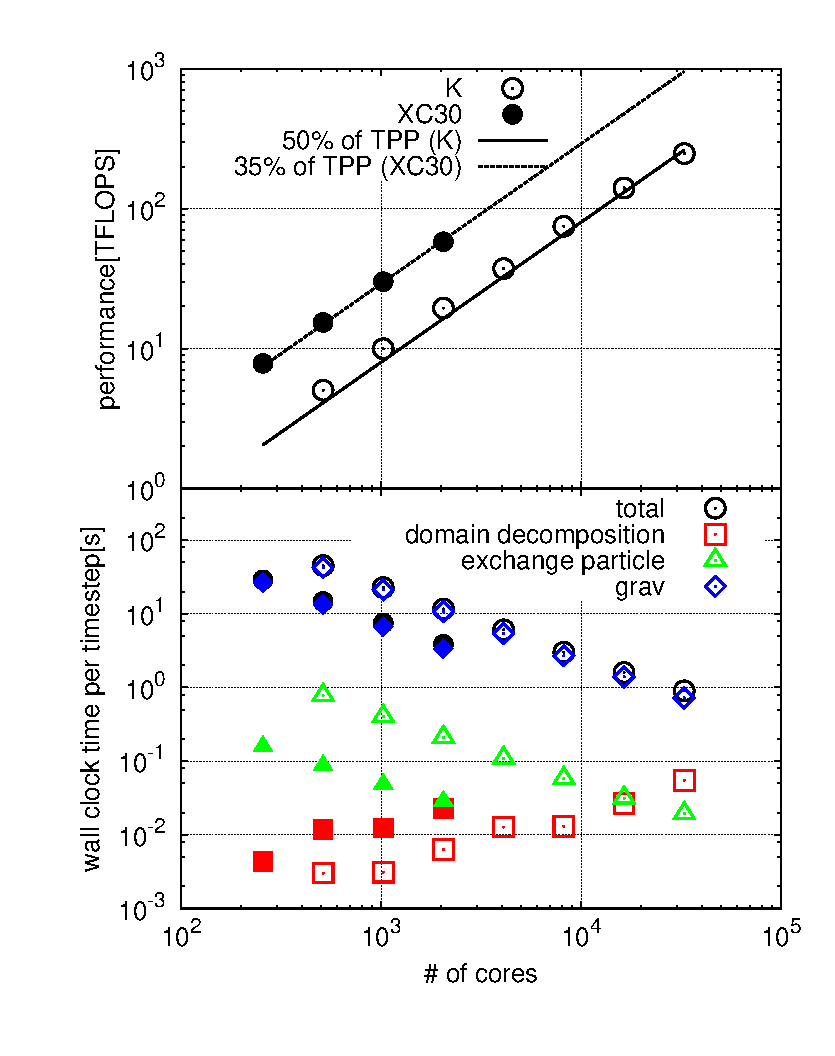
\includegraphics[width=8cm]{figure/disk_strong.eps}
  \end{center}
  \caption{
  
The same figure as figure \ref{fig:disk_weak} but for the
strong-scaling performance for 550 million particles

    }
  \label{fig:disk_strong}
\end{figure}

% LocalWords:  FDPS superparticle monopole quadrupole SIMD builtin Hernquist IC
% LocalWords:  Frenk NFW EP scalability TPP PFLOPS NVIDIA kpc axisymmetric pc
% LocalWords:  GalacticICS Gyrs timestep edorf et al petaflops Wallclock
% LocalWords:  wallclock
